\documentclass[10pt, border=3mm]{standalone}
\usepackage{pstricks-add}
\usepackage{tikz}
\usetikzlibrary{positioning, calc, graphs}

\begin{document}

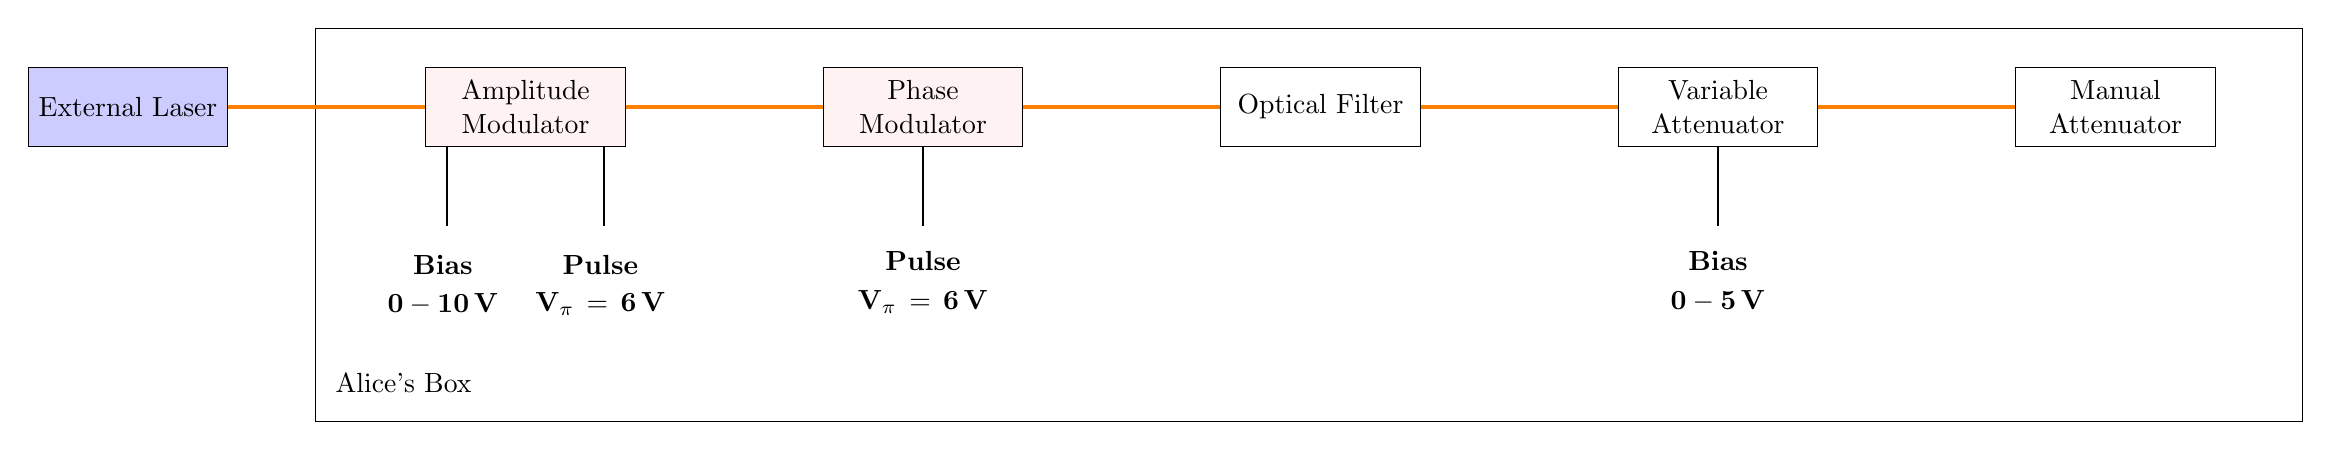
\begin{tikzpicture}[block/.style={rectangle,draw,minimum height=1cm,text width=2.3cm,align=center},node distance = 25mm , block2/.style={-, rectangle,draw,minimum height=5cm,text width=25cm,align=center} ]
\node (b1) [block, fill=blue!20] {External Laser} ;
\node (b2) [block, fill=pink!20, right=of b1] {Amplitude Modulator};
\node (b3) [block, fill=pink!20,right=of b2] {Phase Modulator};
\node (b4) [block,right=of b3] {Optical Filter} ;
\node (b5) [block,right=of b4] {Variable Attenuator};
\node (b6) [block,right=of b5] {Manual Attenuator};
\node (b15) [block2] at (15,-1.5) {};
  \begin{scope}
    \draw [-, orange, very thick] (b1) -- (b2);
    \draw [-, orange, very thick] (b2) -- (b3);
    \draw [-, orange, very thick] (b3) -- (b4);
    \draw [-, orange, very thick] (b4) -- (b5);
    \draw [-, orange, very thick] (b5) -- (b6);
    \draw [-, black, thick] ($(b2.south)+(-1,0)$) -- ($(b2.south)+(-1,-1)$);
    \node (input) at (4,-2){$\mathbf{Bias}$};
    \node (input) at (4,-2.5){$\mathbf{ 0 - 10  \,V}$};

    \draw [-, black, thick] ($(b2.south)+(1,0)$) -- ($(b2.south)+(1,-1)$);
    \node (input) at (6,-2){$\mathbf{Pulse}$};
    \node (input) at (6,-2.5){$\mathbf{ V _\pi \,= \,6 \,V}$}; 
    \draw [-, black, thick] ($(b3.south)+(0,0)$) -- ($(b3.south)+(0,-1)$);
    \node (input) [below  = 1.2cm and -2cm of  b3, name=f]{$\mathbf{Pulse}$};
    \node (input) [below  = 1.7cm and -2cm of  b3, name=f]{$\mathbf{ V _\pi \,= \,6 \,V}$};
    \draw [-, black, thick] ($(b5.south)+(0,0)$) -- ($(b5.south)+(0,-1)$);
    \node (input) [below  = 1.2cm and -2cm of  b5, name=f]{$\mathbf{Bias}$};
    \node (input) [below  = 1.7cm and -2cm of  b5, name=f]{$\mathbf{ 0 - 5  \,V}$};
    \node (input) at (3.5,-3.5){Alice's Box};
  \end{scope}
\end{tikzpicture}
\end{document}